\documentclass{tufte-handout}

\title{On ultimate; O2: secondary middle, left centre or popper}
\author[James Reynolds]{James Reynolds}

%\date{28 March 2010} % without \date command, current date is supplied

%\geometry{showframe} % display margins for debugging page layout

\usepackage{graphicx} % allow embedded images
  \setkeys{Gin}{width=\linewidth,totalheight=\textheight,keepaspectratio}
  \graphicspath{{graphics/}} % set of paths to search for images
\usepackage{amsmath}  % extended mathematics
\usepackage{booktabs} % book-quality tables
\usepackage{units}    % non-stacked fractions and better unit spacing
\usepackage{multicol} % multiple column layout facilities
\usepackage{lipsum}   % filler text
\usepackage{fancyvrb} % extended verbatim environments
  \fvset{fontsize=\normalsize}% default font size for fancy-verbatim environments

% Standardize command font styles and environments
\newcommand{\doccmd}[1]{\texttt{\textbackslash#1}}% command name -- adds backslash automatically
\newcommand{\docopt}[1]{\ensuremath{\langle}\textrm{\textit{#1}}\ensuremath{\rangle}}% optional command argument
\newcommand{\docarg}[1]{\textrm{\textit{#1}}}% (required) command argument
\newcommand{\docenv}[1]{\textsf{#1}}% environment name
\newcommand{\docpkg}[1]{\texttt{#1}}% package name
\newcommand{\doccls}[1]{\texttt{#1}}% document class name
\newcommand{\docclsopt}[1]{\texttt{#1}}% document class option name
\newenvironment{docspec}{\begin{quote}\noindent}{\end{quote}}% command specification environment

\begin{document}

\maketitle% this prints the handout title, author, and date



%\printclassoptions
This document is about 
playing secondary 'middle'
(vertical), 
left-central cutter 
(horizontal), 
or popper 
(zone) 
on offence\footnote{
Referred to here 
as position O2.
This
is part of a series, 
available at
\url{https://github.com/James-Reynolds/Ultimate-strategy-and-tactics}}.
Let the handlers 
deal with catching the pull, but
as you run downfield
try to 
see
what defence structure
is being used. 
%\footnote{It could be:
%person-match defence,
%person-match-last-back-helps,
%person-match-with-a-poacher,
%person-match-with-lots-of switching,
%force-middle,
%force-straight-up,
%zone-3-3-1-force-middle-
%zone-3-3-1-force-sideline
%zone-3-3-1-force-forehand
%zone-3-3-1-force-backhand
%zone-3-3-1-etc
%zone-3-2-2, 
%zone-2-3-2, 
%zone-1-3-2-1 (puppy-fence),
%clam,
%or something else}.

\section{Beating person-match defence with a vertical stack}\label{sec:vertical}

\begin{marginfigure}%
  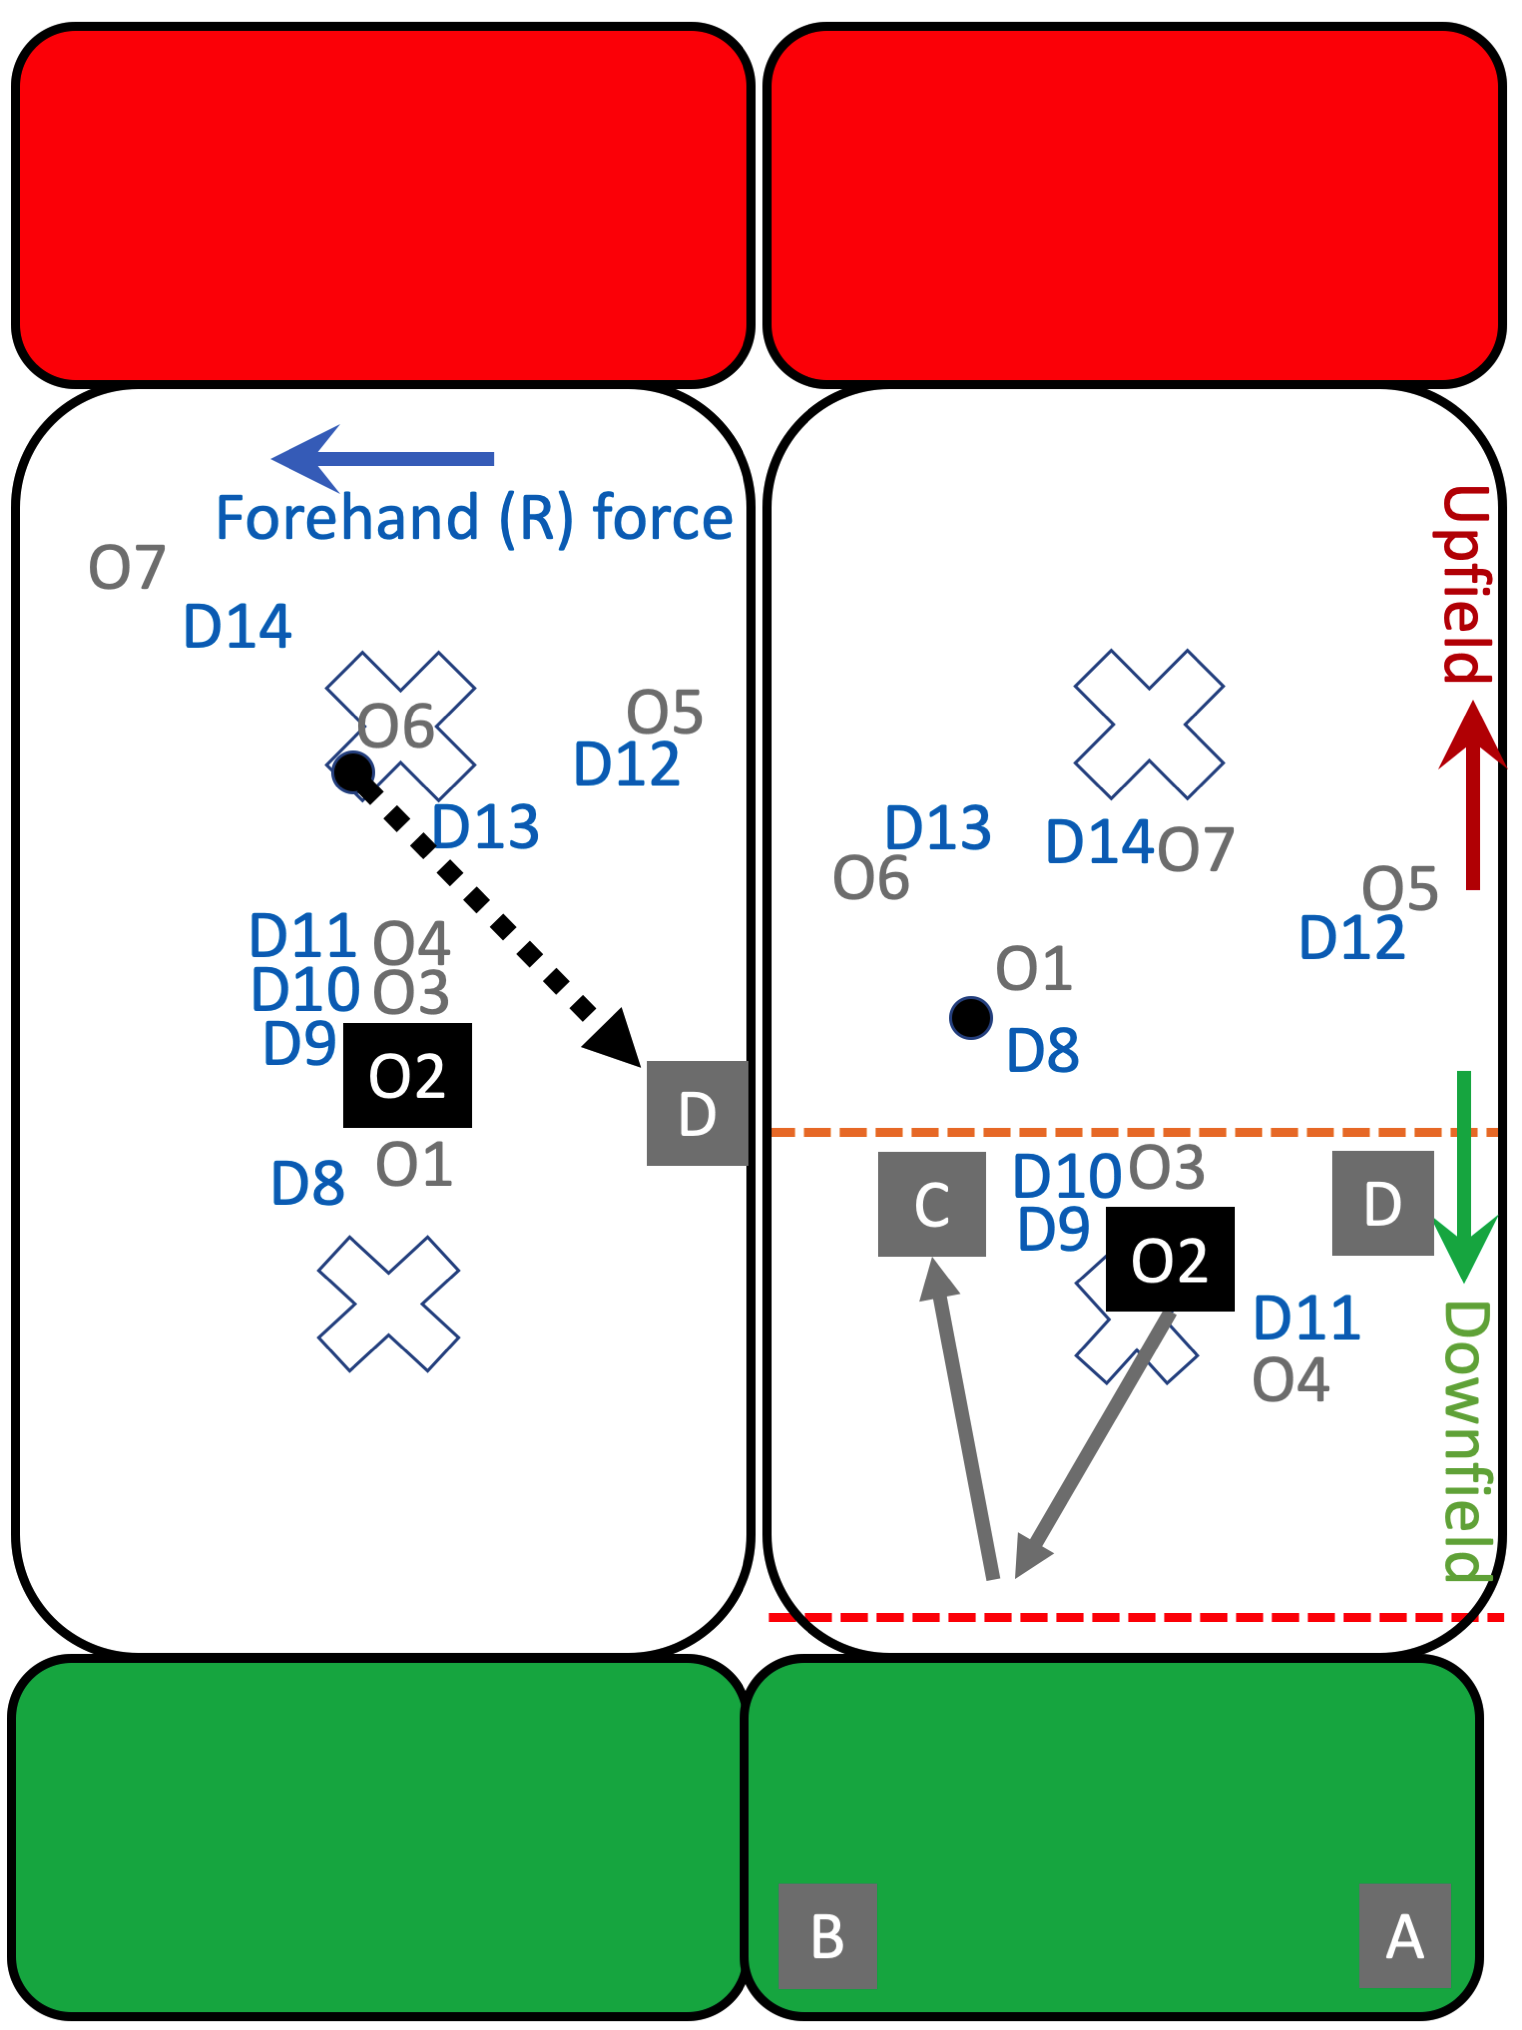
\includegraphics[width=\linewidth]{O2-vertical}
  \caption{Vertical stack: 
  starting position (left),
  and development (right)}
  \label{fig:O2-vertical}
\end{marginfigure}


Figure \ref{fig:O2-vertical} (left) shows 
a situation 
with: 
a brick called;
a forehand force; 
person-match defence; 
and your team using 
a vertical stack formation.
As secondary middle, 
(O2) 
your role 
will likely 
involve cutting 
\smallcaps{after} 
the primary middle 
(O1)\footnote{
Especially as being 
in the middle of the vertical stack,
as shown in 
Figure \ref{fig:O2-vertical} (left)
it is difficult for 
you to make a cut 
without causing 
a pick. 
In contrast, 
Figure \ref{fig:O2-vertical} (right)
shows O1 
having cut upfield 
and received 
a pass 
on the open side, 
which immediately 
frees you 
(O2) 
to cut 
from the back of the stack,
with less chance 
of a pick occuring.}.
However, 
in Figure \ref{fig:O2-vertical} (left)
O6 is shown
potentially throwing 
a break throw to D,
which you 
(O2),
or any of the other cutters
(O1. O3, O4) 
might be able to run onto 
after it is thrown. 
All the defenders 
(D8-D11) 
are on the wrong side, 
so you are all open 
to that space.
However,
you will likely need to 
stay still before it is thrown 
as if you 
cuts towards D 
\smallcaps{prior to the disc being thrown} 
then there is likely 
to be a pick\footnote{
Picks occur
when a  
defender is 
obstructed from 
following someone 
they are marking.  
So maybe stand still
until it's thrown 
so any pick 
might not affect the pass itself
(meaning that it stands), 
and D9 
only gets to catch up 
to put the force on earlier.}.

There are many 
different ways that the 
play might develop.
Figure \ref{fig:O2-vertical} (right) shows 
the disc having been thrown 
to O1
on the back-under 
cut 
to the open side. 
O4 is indicated 
clearing 
or cutting 
deep on 
the break side. 
The stack is shown having 
moved further downfield, 
in response to the pass
to O1
with you, 
having waited
for O1 to cut first,
still in the stack
together with
O3. 
This leaves 
you 
available to make 
cuts
to A-D, 
\smallcaps{now that O1 has the disc.} 


It is this timing 
that is important 
when playing 
in a secondary cutter position. 
O2 is called secondary middle, 
because you cut second, 
not because the position is of secondary importance. 
Ideally,
only  
(maybe) two of the four cutters
(O1-4) 
will be out of the stack (cutting)
at any moment.
Otherwise, 
you will likely 
get in each others way, 
and/or run out of cutters 
in position 
to cut next.  
Staying  
between 
the dashed 
horizontal 
lines 
may also help when cutting\footnote{ 
The position of 
the lines vary
with the position of the disc
and with how far the thrower  
can or will 
throw. 
However, 
if you go 
downfield of the dashed red line 
before the disc is in the air,
D9 may be able 
get to
A or B 
before the disc,
intercepting 
or preventing 
deep throws to 
you or others. 
Similarly, 
if you go 
upfield of the dashed yellow line
then D8 may 
be able to help
prevent dump throws from O6
to O5 
or O7.}.

Vertical works
against other person-match defences. 
But it might need 
some adjustment.
For example
against: (1) RH-backhand-force: mirror the above; 
(2) last-person-covers-the-deepest-threat
you may need to coordinate with O1 
to overload D8 (deep) 
or D9 (under); or
against (3) a straight-up force, 
maybe stay in the stack 
while the handlers move the disc around
until there's an opportunity
for a huck without a marker, 
or if you do cut under 
go out wide 
to the sideline. 


\subsection{Beating person-match defence with feldrunner}
\label{sec:feld}
\begin{marginfigure}%
  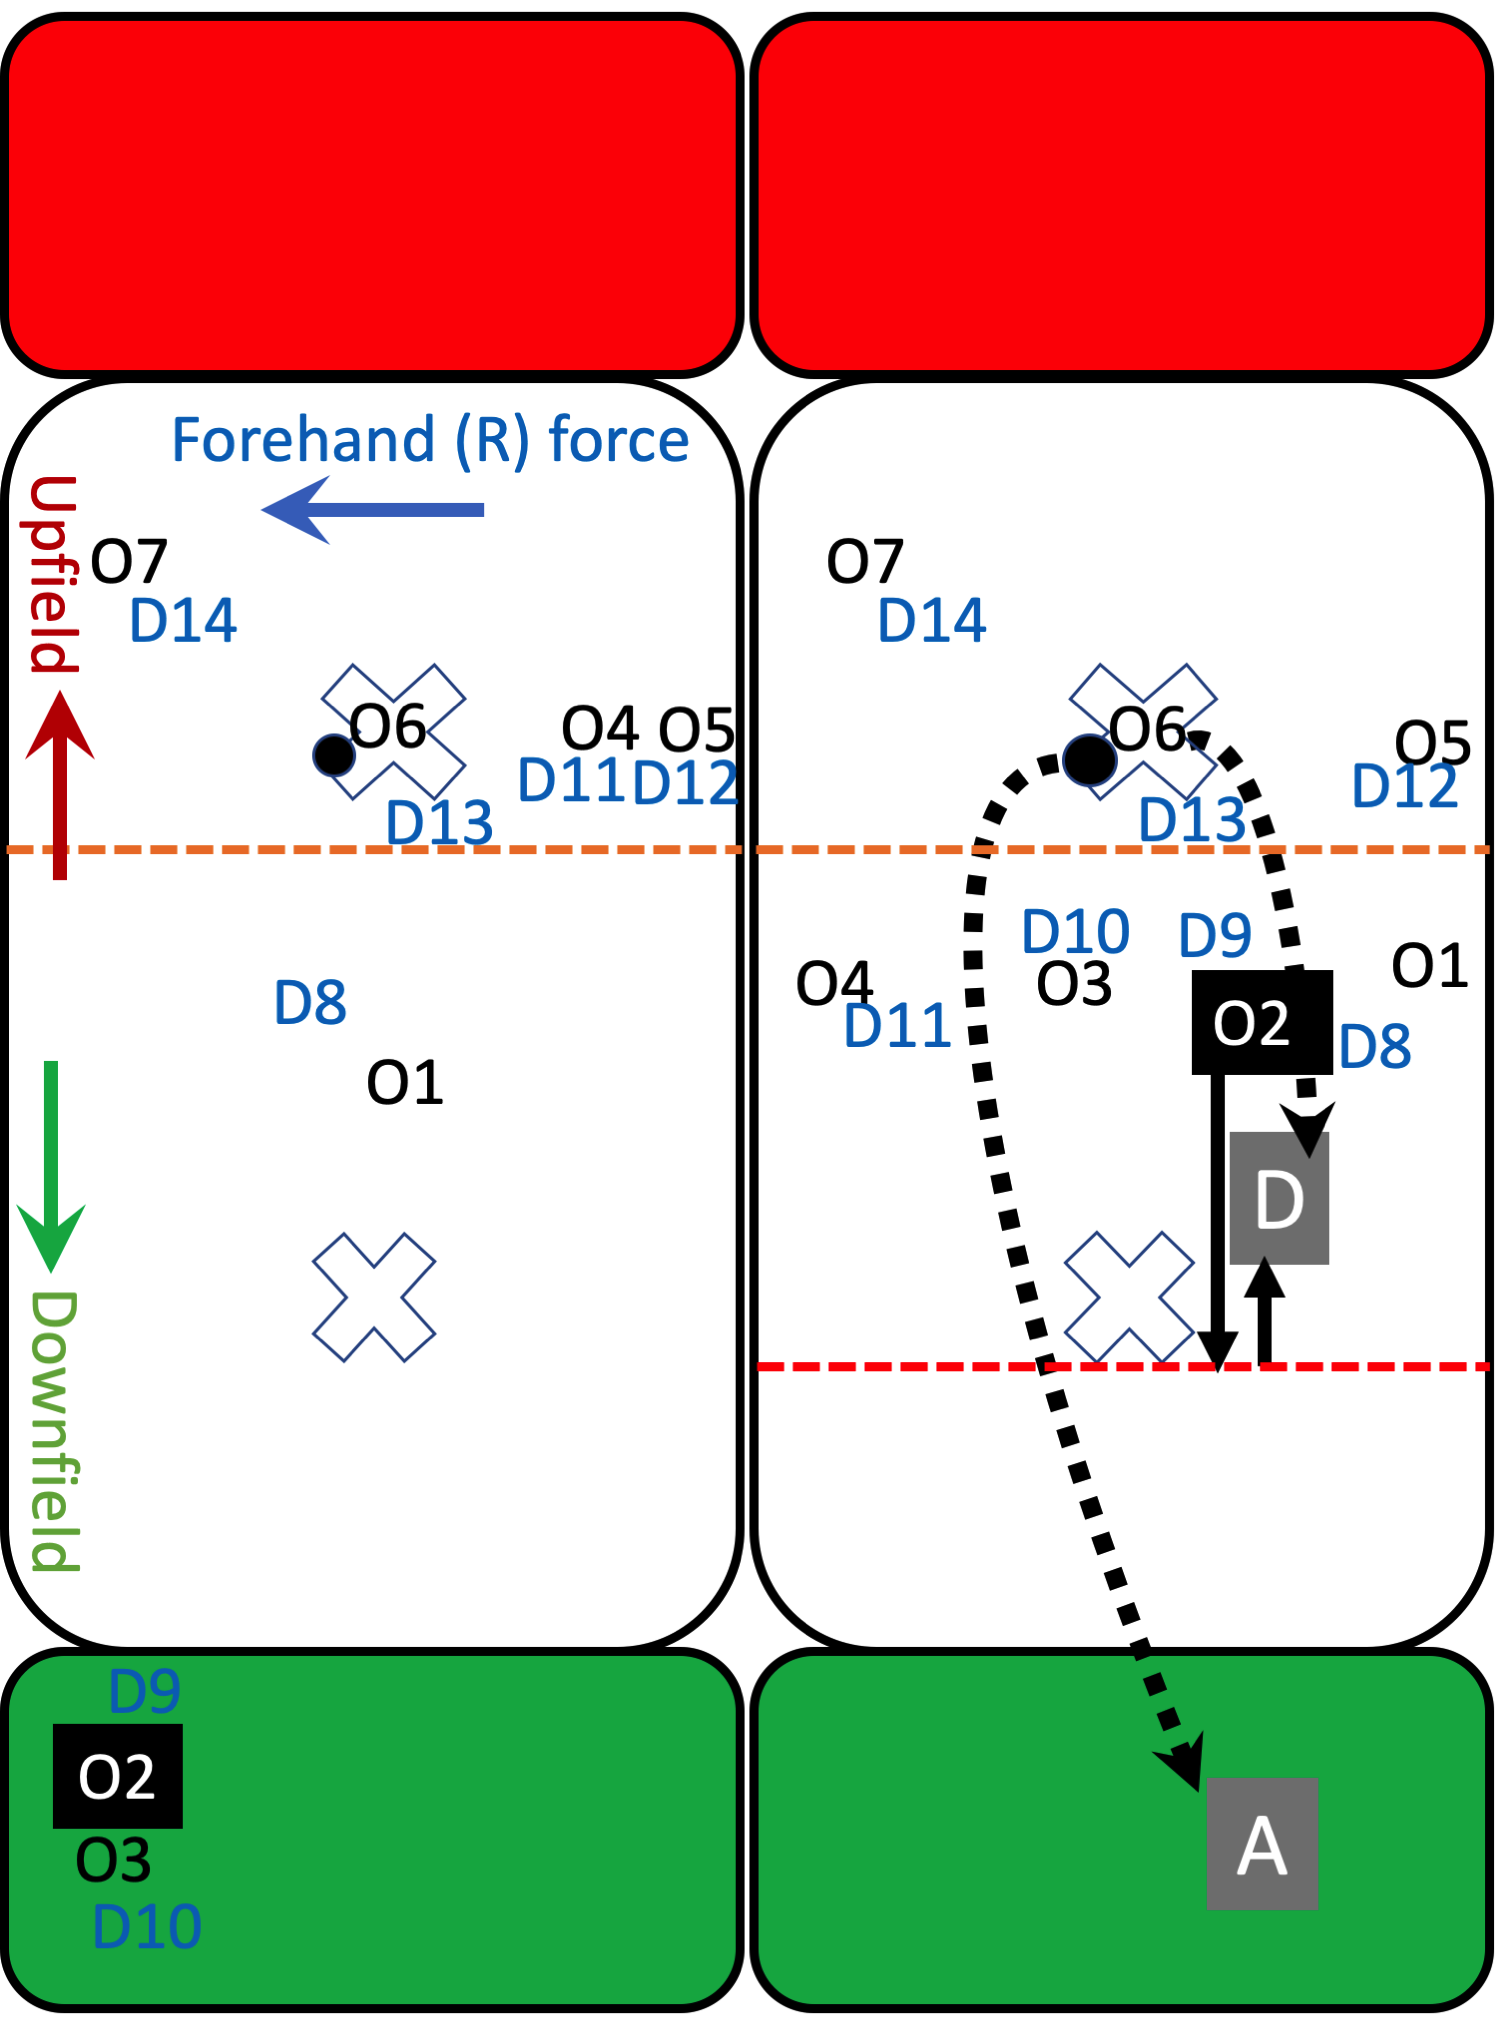
\includegraphics[width=\linewidth]{O2-horizontal}
  \caption{Feldrunner (left) and horizontal (right)}
  \label{fig:O2-horizontal}
\end{marginfigure}
Figure \ref{fig:O2-horizontal} (left) 
shows a feldrunner formation, 
with 4 handlers (O1-4), 
and O1 as the focus.
You  
(O2) 
and O3
are positioned 
together in the endzone.
The idea of feldrunner 
is to pass to 
the isolated
focus. 
They will then either pass to 
O3 or you, 
or dump to the handlers
and reset. 

This formation relies 
on you and O3 
waiting until O1 
gets the disc 
before making a cut.  
It may be that 
one of 
D9 
and D10 
go to help D8 
cover D1.  
If so, 
you and O3 
might spread out, 
one on each side line
and move a bit closer, 
so that one of the handlers
can hit one of you directly 
and quickly. 


\subsection{Beating person-match defence with a horizontal stack}\label{sec:horizontall}
Basic horizontal stack 
involves cutting
upfield and downfield (black arrows)
within your quarter of the field\footnote{
Other cuts
can work, 
but might need
communication,
e.g. diamond cuts 
involve you trading places 
with O1 
or O3.}. 
Figure \ref{fig:O2-horizontal} (right) shows how
O6 
can potentially 
throw to you 
at A 
or D\footnote{
Black arrows
show how a back-under cut 
opens space 
for this throw.}. 

\section{Beating zone defence}\label{sec:zone}

\begin{marginfigure}%
  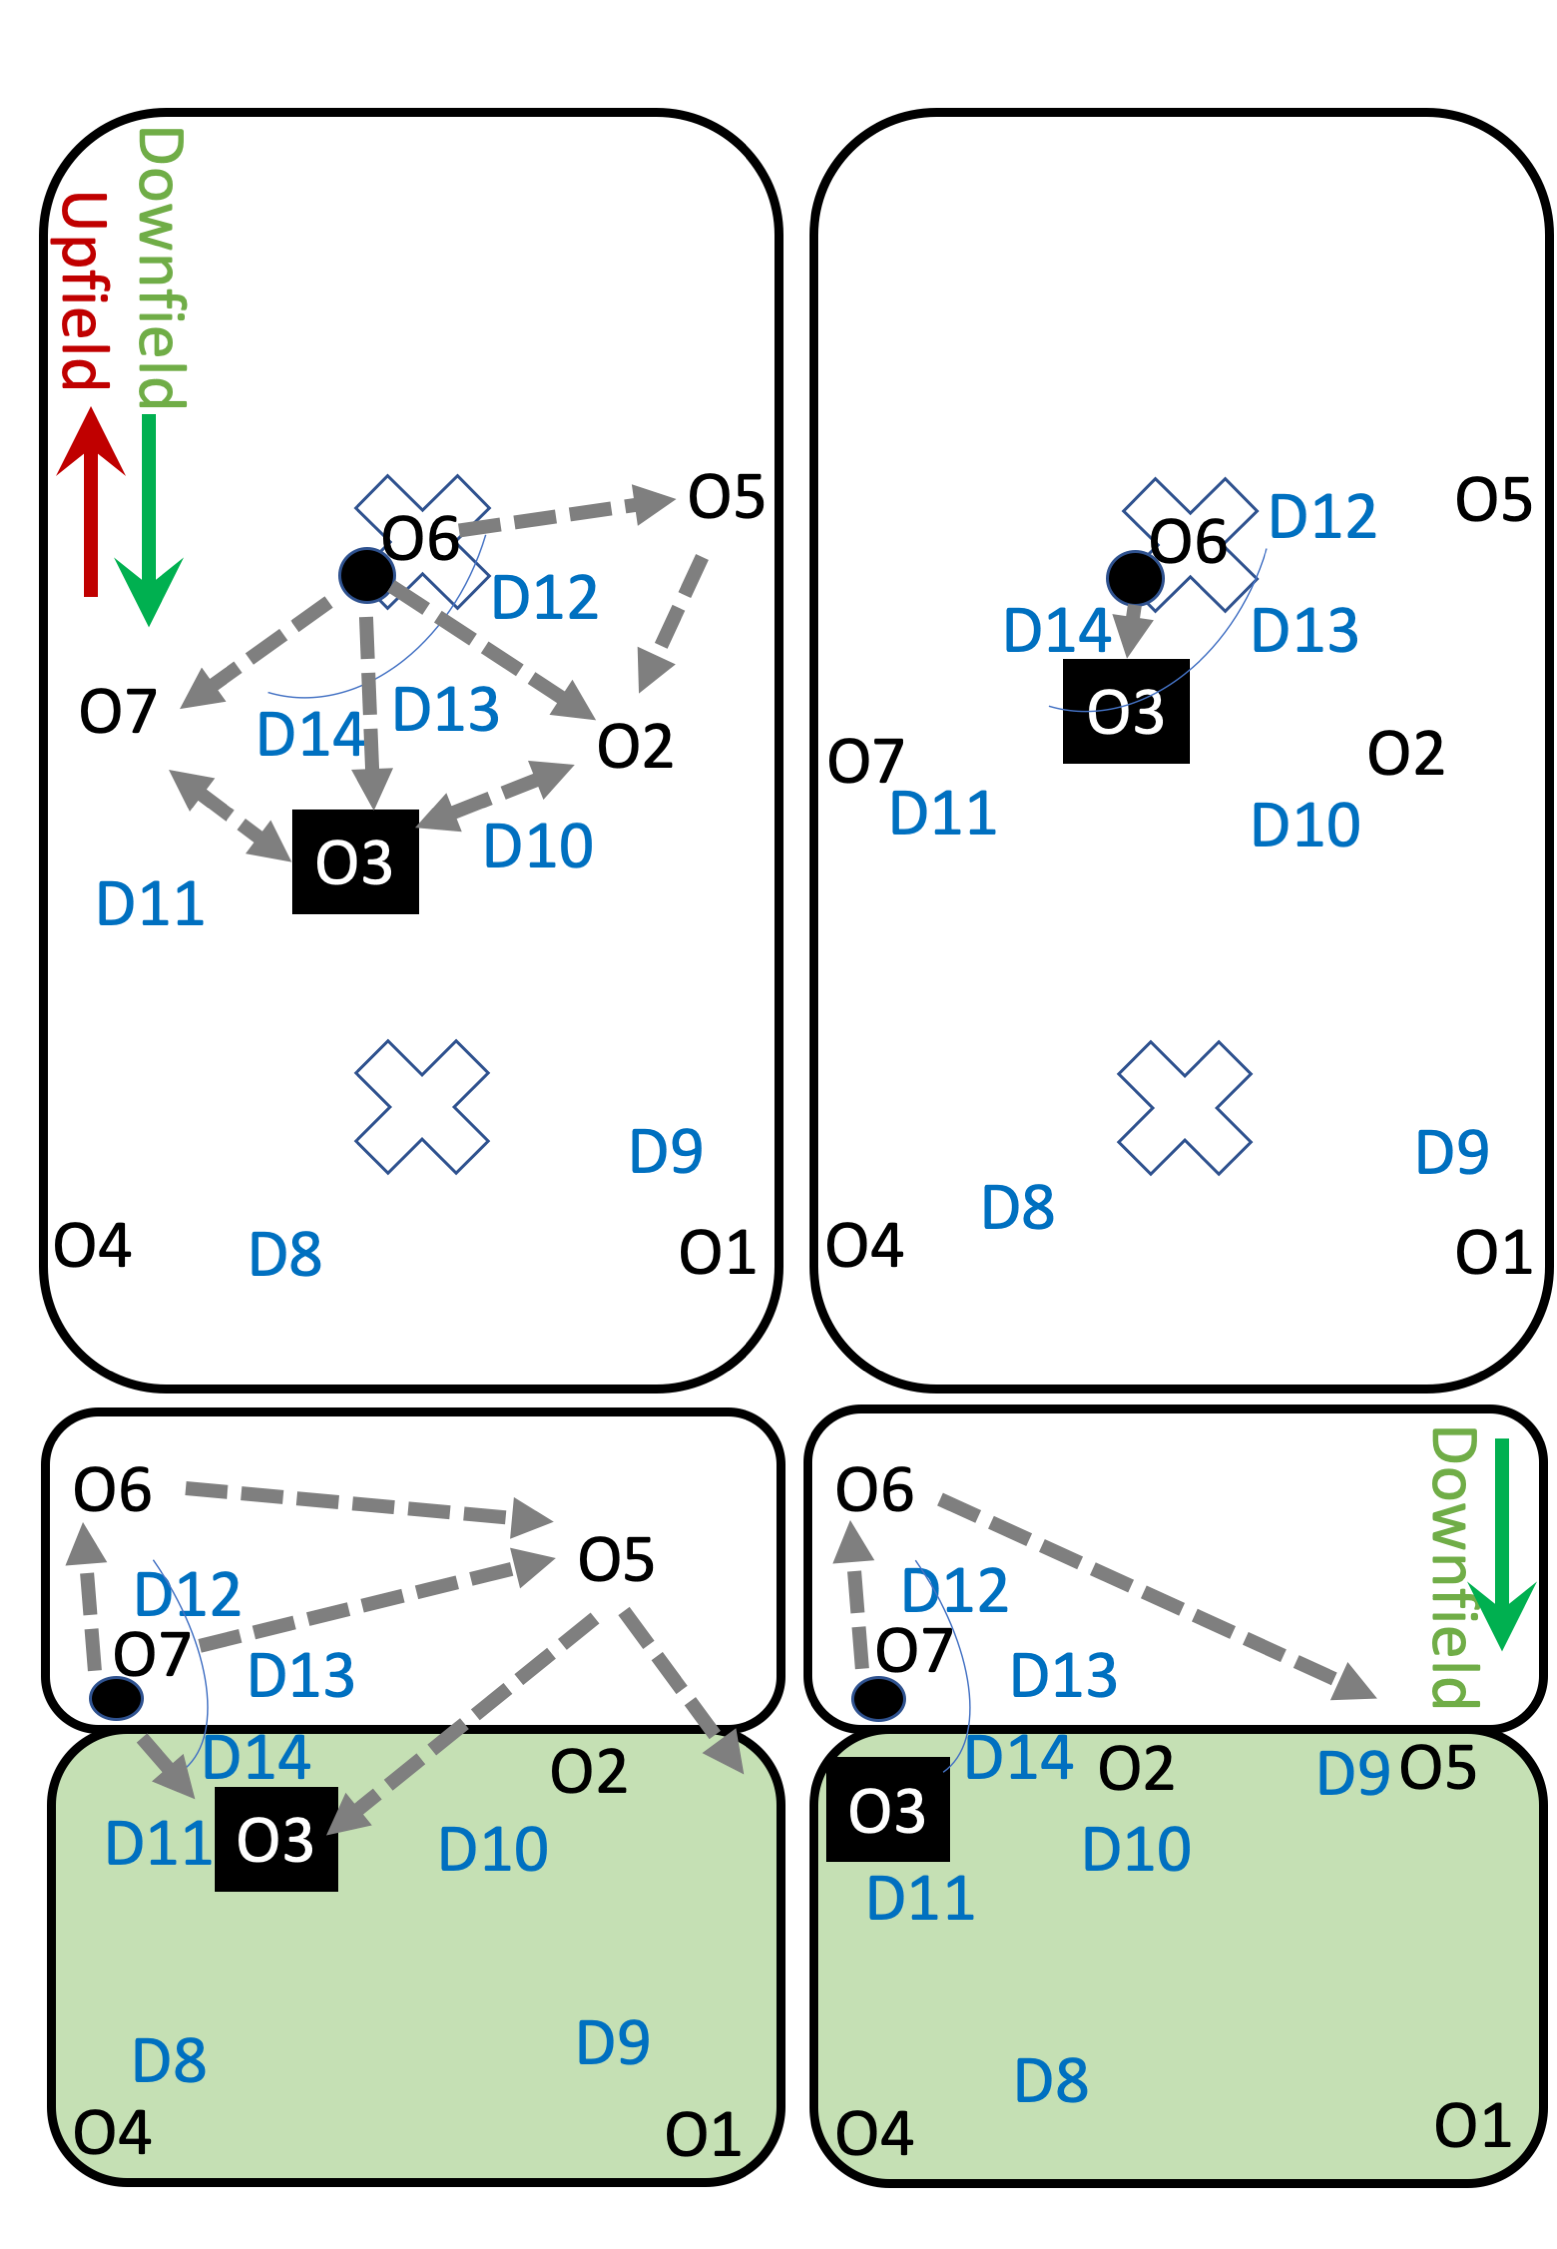
\includegraphics[width=\linewidth]{O2-zone331}
  \caption{formations against 331 zone}
  \label{fig:O2-zone331}
\end{marginfigure}

Vertical stack 
probably won't work. 
Instead, your 
team needs to 
spread out. 
Three ways to beat a zone are:
(1) over;
(2) round; or
(3) through. 
Figure \ref{fig:O2-zone331}
(top left)
shows this 
against a 
3-3-1 zone, 
with you 
behind the cup  
O6 might then
be able to throw 
through 
the gap between 
D12 
and D13, or 
over the cup\footnote{
short hammer, scoober.}, 
to get the disc to you. 
Alternatively, 
it might go round to 
O5 and then to you.

An issue 
to keep in mind 
is how you and O3
coordinate to split 
D10. 
In Figure \ref{fig:O2-zone331}
(top left), 
D10 is shown as having to 
try to cover both 
you and O3, 
with perhaps some help 
from D9 
and D11. 
In contrast, 
Figure \ref{fig:O2-zone331}
(top right) 
show a position 
that might occur 
if you `crash' 
the cup\footnote{ 
This style of play 
might be used 
to disrupt the 
cup's formation, and 
reset the stall count 
with a short pass. 
I'm not a huge fan, 
unless its one of the handlers 
crashing from behind.}
However, 
this might allow D10 
to ignore you 
and play 
tighter on O3\footnote{ 
It might also allow 
D9 to threaten to intercept 
a pass to O5 
(blue arrow), 
and have further,
cascading, 
impacts. 
In general, 
by crashing the cup
from downfield 
it becomes 3 (O1, O3 and O4) 
versus 4 (D8-11) 
downfield of the cup, 
which is not ideal.}. 
An exception, 
however,,
is shown in 
Figure \ref{fig:O2-zone331}
(bottom right), 
where close to the endzone 
moving in towards 
the cup 
might suck D10 
in as well, 
opening more space for O5 
in the front corner.  
Alternatively, 
Figure \ref{fig:O2-zone331}
(bottom left), 
indicates how spreading 
might split D10, 
so that if it gets to 
O5 
they can then score to 
either O2 
or O3. 


\section{Beating clam defence}\label{sec:zone}
Clam mixes person-match 
and zone defence styles\footnote{
Involves defenders 
switching 
so as to cover 
an area. 
For example, 
in Figure \ref{fig:O2-vertical}(left) 
D8 
(the deep-deep) 
might cover 
O1 deep, 
but then switch with D11 
(open-side wing)
to cover O4's cut deep, 
while D11 covers 
the O1 
cut to C.}.
Whereever you cut, 
one or more defenders
will likely have you
(at least somewhat) covered. 
As O2, 
you might
coordinate 
with O1
to overload
D8 or D9.



\end{document}
